%!TEX root = ../main.tex
\chapter{Contribution}\label{chap:contribution}
\section{Notation}
In the following we will use the notation:
\begin{align*}
	\mathbb{I} \left(X , Y; D, P_M, C_M \right)
\end{align*}
which expresses the mutual information between $X$ and $Y$ and $D, P_M, C_M$, separated by a semi-colon, are the trainable parameters of the system. The parameters can be seen as additional input to a function.
\section{First implementation}
In this section we break-down the autoencoder system presented by Aref et. al. in \cite{Aref}.
\subsection{Optimization of trainable parameters}
As we have seen in chapter \ref{chap:preliminaries}, the goal of probabilistic constellation shaping is to maximize the mutual information
\begin{align}
	 \max_{D, P_M, C_M} \mathbb{I} \left(X , Y ; D, P_M, C_M \right) \overset{\text{(a)}}{=} \mathbb{H}(X) - \mathbb{X}(P_{X|Y} \Vert Q_{X|Y} ; D, P_M, C_M)
\end{align}

where the entropy is maximized when the symbols probabilities follow a \cGls{mb} distribution; and the cross-equivocation is minimum when $Q_{X|Y} = P_{X|Y}$.

Typically, the gradient descent (or ascent, as we intent to maximize) allows us to solve the optimization problem by adjusting the trainable parameters as:
\begin{align}
	\theta_{new} = \theta_{old} + \epsilon \pdv{\theta_{old}} \mathbb{I} \left(X , Y ; \theta_{old} \right)
\end{align}
for all trainable parameters $\theta \in P_M, C_M, D$. And the \cGls{mi} can be numerically approximated by
\begin{align}
	\mathbb{I} \left(X , Y\right) \approx \mathbb{I} \left(X , Y\right)_{\text{num}} &= \dfrac{1}{B} \sum \limits_{i = 1}^{B} - \log_2(P(x_i)) + \log_2(Q_{X|Y}(x_i|y_i))\\
	&= \dfrac{1}{B} \sum \limits_{i = 1}^{B} L(x_i, y_i).
\end{align}

Next, the following approximation usually allows to adjust the trainable parameters:
\begin{align}
	\pdv{\theta} \mathbb{I} \left(X , Y ; \theta \right) \approx \pdv{\theta} \mathbb{I} \left(X , Y\right)_{\text{num}} = \dfrac{1}{B} \sum \limits_{i = 1}^{B} L(x_i, y_i).
\end{align}

However, Aref claims that although this is true for the constellation locations $(\theta \in C_M)$ and the demapper parameters $(\theta \in D)$, it does not hold for the constellation probabilities $\{p_1, p_2, \dots, p_M\} = P_M$
\begin{align}
\label{eqn:mi_pdv_p}
	\pdv{p_j} \mathbb{I} \left(X , Y ; P_M \right) \not\approx \dfrac{1}{B} \sum \limits_{i = 1}^{B} \pdv{p_j} L(x_i, y_i)
\end{align}

as $\{p_1, p_2, \dots, p_M\}$ changes the statistics of the training set.

For this reason, \ref{eqn:mi_pdv_p} must be computed differently. On the one hand, to compute the derivative of the cross-equivocation, the following expansions are useful
\begin{align}
	\mathbb{X}\left(P_{X|Y} \Vert Q_{X|Y} \vert Y=b \right) = \sum \limits_{a \in Supp(P_{X|Y}(\cdot|b))} P_{X|Y}(a|b) \log_2(Q_{X|Y}(a|b))
\end{align}

\begin{align}
	\mathbb{X}\left(P_{X|Y} \Vert Q_{X|Y}\right) = \sum \limits_{b \in Supp(P_Y)} P_Y(b) \mathbb{X}\left( P_{X|Y} \Vert Q_{X|Y} \vert Y=b \right) 
\end{align}

as combined together and applying Bayes' theorem they yield

\begin{align}
\label{eqn:CE_expanded}
	\mathbb{X}\left(P_{X|Y} \Vert Q_{X|Y}\right) = \sum \limits_{(a,b) \in Supp(P_{XY})} P_X(a) P_{Y|X}(b|a) \log_2(Q_{X|Y}(a|b)). 
\end{align}

And so, the derivative results
\begin{align}
	\pdv{p_j} \mathbb{X}\left(P_{X|Y} \Vert Q_{X|Y}\right) &= \sum \limits_{b \text{ if } x=j} P_{Y|X}(b|j) \log_2 Q_{X|Y}(j|b) \\
	& + \sum \limits_{(a,b) \in Supp(P_{XY})} P_{XY}(a, b) \pdv{p_j} \log_2 Q_{X|Y}(a|b)
\end{align}
which can be rewritten using the expectation operator as
\begin{align}
	\pdv{p_j} \mathbb{X}\left(P_{X|Y} \Vert Q_{X|Y}\right) &= \mathbb{E}_{Y|X}[ \log_2 Q_{X|Y}(j|b)| X=j] \\
	& + \mathbb{E}_{XY}[ \pdv{p_j} \log_2 Q_{X|Y}(a|b)].
\end{align}
The terms can now be numerically computed as
\begin{align}
\label{eqn:CE_term_1}
	\mathbb{E}_{Y|X}[ \log_2 Q_{X|Y}(j|b)| X=j] \approx \dfrac{1}{Bp_j}\sum \limits_{b \text{ if } x=j} \log_2 Q_{X|Y}(j|b)
\end{align}
\begin{align}
\label{eqn:CE_term_2}
	\mathbb{E}_{XY}[ \pdv{p_j} \log_2 Q_{X|Y}(a|b)] \approx \dfrac{1}{B} \sum \limits_{(a,b) \in Supp(P_{XY})} \log_2 Q_{X|Y}(a|b).
\end{align}
On the other hand, the derivative of the entropy w.r.t. $p_j$ is
\begin{align}
\label{eqn:H_term_1}
	\pdv{p_j} \mathbb{H}(X) = \pdv{p_j} \sum \limits_{i = 1}^{B} - p_i \log_2(p_i) = - \log_2 (p_j) - log_2 (e).
\end{align}

Now, combining \ref{eqn:CE_term_1}, \ref{eqn:CE_term_2}, and \ref{eqn:H_term_1} the derivative of the mutual information w.r.t. $p_j$, \ref{eqn:mi_pdv_p}, can be computed as
\begin{align}
	\pdv{p_j} \mathbb{I} \left(X , Y ; P_M \right) \approx - \log_2 (p_j) - \log_2 (e) + \dfrac{1}{Bp_j}\sum \limits_{b \text{ if } x=j} \log_2 Q_{X|Y}(j|b) + \dfrac{1}{B} \sum \limits_{(a,b)} \log_2 Q_{X|Y}(a|b)
\end{align}

Aref now indicates that the following terms can be computed via backpropagation
\begin{align}
	- \log_2 (p_j) + \dfrac{1}{Bp_j}\sum \limits_{b \text{ if } x=j} \log_2 Q_{X|Y}(j|b) = \dfrac{1}{B} \sum \limits_{i = 1}^{B} \pdv{p_j} L(x_i, y_i)
\end{align}
while the remaining ones must be explicitely computed and added to the gradient after backpropagating. We call this step \textit{gradient correction} and it is due to the change of statistics in the sampled batch.

\subsection{End-to-End System architecture}
\begin{figure}[h!]
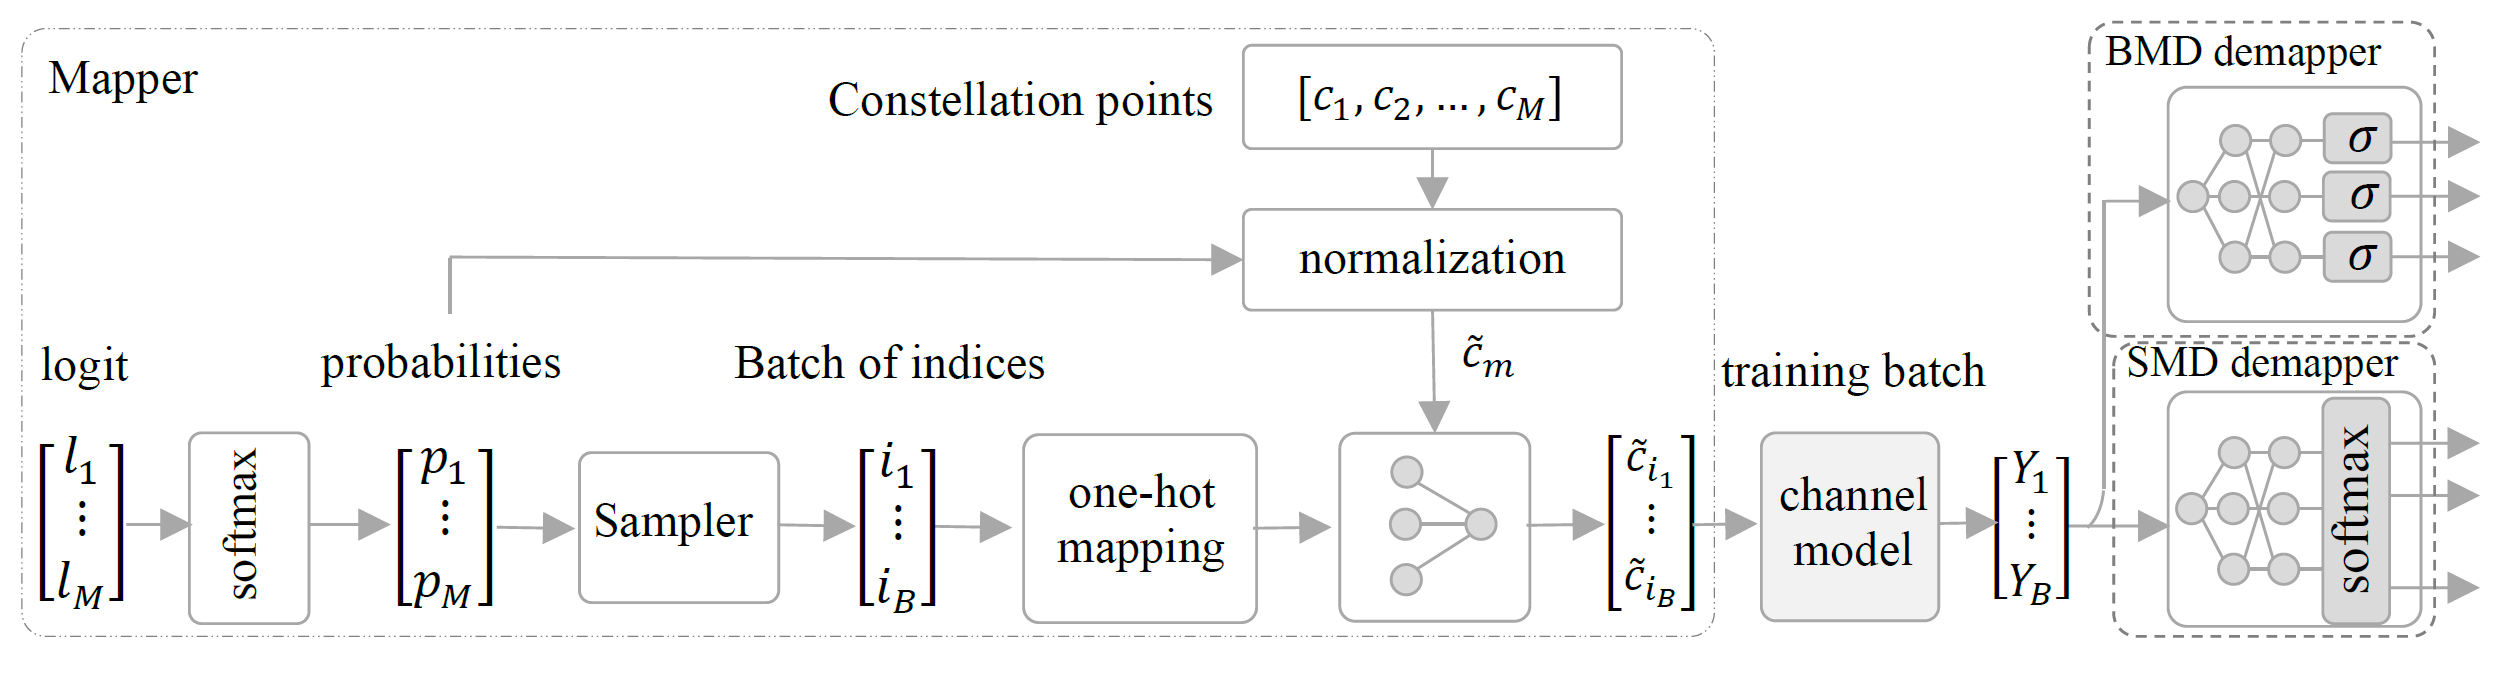
\includegraphics[width=\textwidth]{figs/aref_diagram.png}
\centering
\end{figure}

\section{Second implementation}
In this section we break-down the autoencoder system presented by Stark et. al. in \cite{Stark}.
\subsection{Optimization of trainable parameters}
As in the first implementation Stark also intents to maximize the mutual information. However, the reasoning leading to the definition of the loss function is slightly different. Starting from the demodulator, the categorial cross entropy loss
\begin{align}
	L(D, P_M, C_M) \triangleq \mathbb{X}(P_{X|Y}||Q_{X|Y}; D) = \mathbb{E}\left[-\log_2(Q(X|Y;D))\right] 
\end{align}


is appropriate for training $D$. In addition, the following expansions will come handy
\begin{align}
	\mathbb{H}(X) = \mathbb{X}(P_{X|Y}||Q_{X|Y}) - \mathbb{D}(P_{X|Y}||Q_{X|Y})
\end{align}
\begin{align}
	\mathbb{H}(X|Y=y) = \mathbb{X}(P_{X|y}||Q_{X|y}|Y=y) - \mathbb{D}(P_{X|y}||Q_{X|y}|Y=y)
\end{align}
\begin{align}
	\mathbb{H}(X|Y) = \mathbb{E}_y\left[\mathbb{X}(P_{X|y}||Q_{X|y}|Y=y)\right] - \mathbb{E}_y \left[\mathbb{D}(P_{X|y}||Q_{X|y}|Y=y)\right].
\end{align}
Using the last expansion we can rewrite the mutual information in terms of the categorical cross entropy
\begin{align}
	\mathbb{I} \left(X , Y\right) = \mathbb{H}(X) - \mathbb{X}(P_{X|Y}||Q_{X|Y}) + \mathbb{D}(P_{X|Y}||Q_{X|Y}).
\end{align}
And the loss function becomes 
\begin{align}
	L(D, P_M, C_M) \triangleq \mathbb{H}(X) - \mathbb{I} \left(X , Y\right) + \mathbb{D}(P_{X|Y}||Q_{X|Y}).
\end{align}
So, if $L$ is minimized during training, the source entropy is unwantedly as well minimized. To avoid this effect, Sark et. al defines a new loss function
\begin{align}
	\hat{L}(D, P_M, C_M) \triangleq L(D, P_M, C_M) - \mathbb{H}(X).
\end{align}
We can now see the optimization problem as
\begin{align}
	\min_{D, P_M, C_M}\hat{L}(D, P_M, C_M) = \max_{D, P_M, C_M} \{ \mathbb{I} \left(X , Y\right) - \mathbb{D}(P_{X|Y}||Q_{X|Y})\}.
\end{align}

\subsection{End-to-End System architecture}
\begin{figure}[h!]
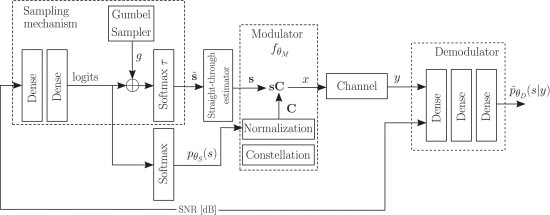
\includegraphics[width=\textwidth]{figs/stark_diagram.png}
\centering
\end{figure}

